\subsection{Thiết kế AI Agent}
\subsubsection{Lựa chọn kiến trúc cho AI Agent}
Trợ lý Ảo trong dự án không chỉ thực hiện chức năng hội thoại tư vấn mà còn trực tiếp tham gia vào các nghiệp vụ khác như đặt hàng và hủy đơn. Do đó, kiến trúc AI Agent cần được thiết kế theo hướng hiện đại, linh hoạt và có khả năng mở rộng, đáp ứng đồng thời các yêu cầu kỹ thuật và nghiệp vụ sau:
\begin{itemize}
    \item Hỗ trợ \textbf{nhiều loại tác vụ khác nhau}, bao gồm cả tác vụ không có side-effect (tư vấn, hỏi đáp) và tác vụ có side-effect (đặt hàng, hủy đơn).
    \item Đảm bảo \textbf{phản hồi theo thời gian thực (real-time)} để mang lại trải nghiệm hội thoại tự nhiên và liền mạch cho người dùng.
    \item Hỗ trợ \textbf{hội thoại không tuyến tính}, cho phép người dùng thay đổi ý định, chen ngang câu hỏi hoặc quay lại tác vụ trước đó trong cùng một phiên làm việc.
    \item Đảm bảo \textbf{an toàn nghiệp vụ}, tránh việc mô hình ngôn ngữ tự ý thực hiện các hành động nhạy cảm ảnh hưởng đến trạng thái hệ thống.
    \item Cho phép \textbf{mở rộng và bảo trì độc lập}, có thể bổ sung luồng nghiệp vụ hoặc agent mới mà không ảnh hưởng đến toàn bộ hệ thống.
    \item Dễ dàng \textbf{kiểm soát, theo dõi và giải thích luồng xử lý}, phục vụ cho việc debug.
\end{itemize}

Từ các yêu cầu trên có thể thấy, kiến trúc AI Agent cần có khả năng điều phối linh hoạt, mức độ kiểm soát cao và không phù hợp với các mô hình agent đơn giản hoặc xử lý tập trung. Sau khi nghiên cứu và so sánh các kiến trúc cho Agent theo hướng Single-Agent và Multi-Agent, nhóm lựa chọn kiến trúc \textbf{Multi-Agent kiểu Hierarchical Supervisor} cho hệ thống Trợ lý Ảo AI vì các lý do sau:
\begin{itemize}
    \item Phù hợp với hệ thống có \textbf{nhiều luồng nghiệp vụ khác nhau}, mỗi luồng có mức độ rủi ro và yêu cầu kiểm soát riêng.
    \item Cho phép \textbf{phân tách trách nhiệm rõ ràng} giữa các agent chuyên môn, giúp giảm độ phức tạp của từng agent.
    \item \textbf{Supervisor Agent đóng vai trò điều phối trung tâm}, giúp kiểm soát luồng hội thoại, tránh xung đột khi nhiều intent xuất hiện đồng thời.
    \item Dễ dàng \textbf{kiểm soát và giải thích luồng xử lý}, đặc biệt quan trọng trong các nghiệp vụ thương mại điện tử có quy trình tuần tự và điều kiện rõ ràng.
    \item Tăng \textbf{độ an toàn của hệ thống}, đặc biệt đối với các tác vụ có side-effect như đặt hàng và hủy đơn.
    \item Hỗ trợ \textbf{mở rộng linh hoạt}, cho phép thay đổi hoặc nâng cấp kiến trúc bên trong từng agent mà không ảnh hưởng đến toàn bộ hệ thống.
\end{itemize}

Với những ưu điểm trên, kiến trúc Multi-Agent kiểu Hierarchical Supervisor đáp ứng tốt các yêu cầu về an toàn, khả năng mở rộng và kiểm soát nghiệp vụ của hệ thống.





\subsubsection{Tổng quan kiến trúc AI Agent}
\begin{figure}[H]
    \centering
    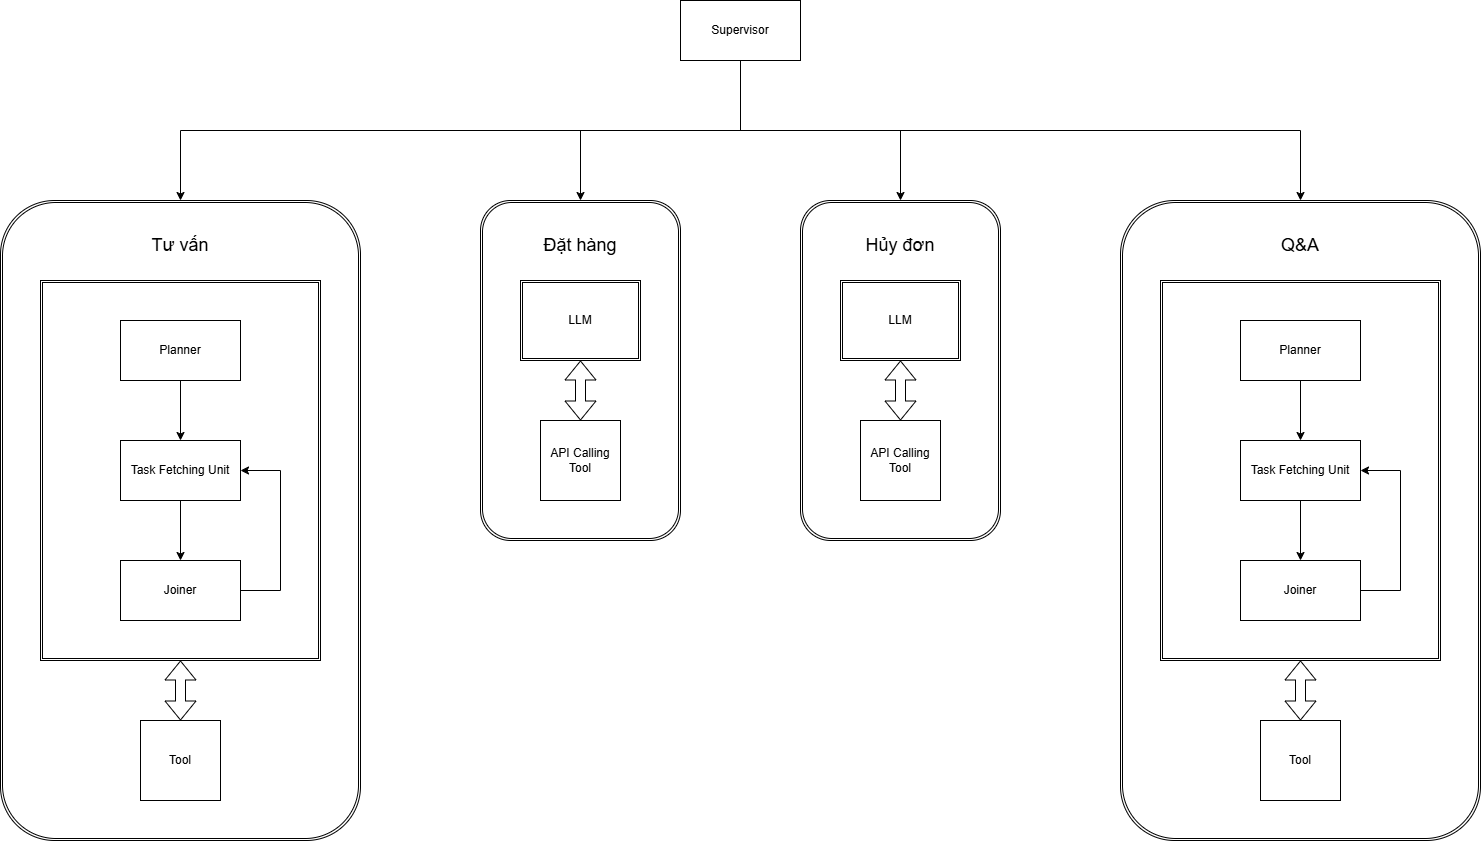
\includegraphics[width=\textwidth]{images/chap6/AI Agent architecture.drawio.png}
    \vspace{0.5cm}
    \caption{Sơ đồ kiến trúc AI Agent}
    \label{fig:ai_agent_architecture}
\end{figure}

Dựa trên kiến trúc đã lựa chọn, hệ thống Trợ lý Ảo AI được thiết kế như hình \ref{fig:ai_agent_architecture}, bao gồm:
\begin{itemize}
    \item Một \textbf{Supervisor Agent} đóng vai trò điều phối cấp cao.
    \item Bốn \textbf{Agent chuyên môn}, tương ứng với bốn luồng nghiệp vụ chính:
    \begin{itemize}
        \item Tư vấn sản phẩm
        \item Đặt hàng
        \item Hủy đơn
        \item Hỏi đáp (Q\&A)
    \end{itemize}
\end{itemize}

Supervisor Agent tiếp nhận yêu cầu từ người dùng, phân tích intent và quyết định agent chuyên môn phù hợp để xử lý. Các agent chuyên môn hoạt động độc lập, tập trung vào nghiệp vụ của mình, nhưng luôn chịu sự giám sát và điều phối của Supervisor.

Cách tổ chức này giúp hệ thống vừa đảm bảo tính linh hoạt của hội thoại tự nhiên, vừa duy trì được mức độ kiểm soát cần thiết đối với các nghiệp vụ quan trọng của thương mại điện tử.

\textbf{Supervisor Agent}

Supervisor Agent là thành phần trung tâm của kiến trúc, chịu trách nhiệm:
\begin{itemize}
    \item Tiếp nhận và phân tích yêu cầu từ người dùng.
    \item Xác định intent hiện tại của hội thoại.
    \item Điều phối và kích hoạt agent chuyên môn tương ứng.
    \item Theo dõi trạng thái thực thi và kiểm soát luồng xử lý tổng thể.
\end{itemize}
Supervisor \textbf{không trực tiếp thực hiện nghiệp vụ}, mà chỉ đóng vai trò điều phối và giám sát. Thiết kế này giúp tránh việc một agent phải xử lý nhiều loại tác vụ khác nhau, đồng thời tăng khả năng kiểm soát và mở rộng hệ thống.


\textbf{Luồng Tư vấn -- LLMCompiler Agent}

Agent tư vấn được thiết kế theo mô hình \textbf{LLMCompiler}, phù hợp với các nhiệm vụ yêu cầu khả năng suy luận nhiều bước và tổng hợp thông tin từ nhiều nguồn khác nhau. Luồng này tập trung vào việc hỗ trợ người dùng lựa chọn sản phẩm phù hợp dựa trên nhu cầu, ngân sách và sở thích cá nhân.

Do đặc thù của nghiệp vụ tư vấn là các câu hỏi mở, không có quy trình cố định và không gây tác động trực tiếp đến trạng thái hệ thống, việc sử dụng LLMCompiler giúp tối ưu khả năng lập kế hoạch, truy xuất thông tin và tổng hợp câu trả lời một cách linh hoạt. Cấu trúc nội bộ của luồng này bao gồm:
\begin{itemize}
    \item \textbf{Planner}: phân tích yêu cầu tư vấn của người dùng và chia nhỏ thành các nhiệm vụ con.
    \item \textbf{Task Fetching Unit}: thực hiện truy xuất dữ liệu (ví dụ: thông tin sản phẩm, so sánh cấu hình).
    \item \textbf{Joiner}: tổng hợp kết quả từ các nhiệm vụ con thành câu trả lời hoàn chỉnh.
    \item \textbf{Tool}: truy cập nguồn dữ liệu bên ngoài như cơ sở dữ liệu sản phẩm và hệ thống RAG.
\end{itemize}
Việc lựa chọn LLMCompiler cho luồng tư vấn giúp hệ thống nâng cao chất lượng reasoning, đồng thời đảm bảo an toàn do không phát sinh side-effect lên hệ thống nghiệp vụ.


\textbf{Luồng Đặt hàng -- ReAct Agent}

Agent đặt hàng được thiết kế theo mô hình \textbf{ReAct}, phù hợp với các nghiệp vụ có trạng thái kéo dài và phát sinh side-effect. Trong luồng này, trợ lý ảo không chỉ suy luận mà còn cần thực hiện các hành động cụ thể bao gồm: kiểm tra còn hàng tồn và tạo đơn hàng thông qua các dịch vụ backend.

ReAct cho phép agent hoạt động theo vòng lặp Reason $ \rightarrow $ Act $ \rightarrow $ Observe, nhờ đó có thể kiểm soát chặt chẽ từng bước trong quy trình đặt hàng và đảm bảo các điều kiện nghiệp vụ được thỏa mãn trước khi thực hiện hành động. Cấu trúc nội bộ của luồng này bao gồm:
\begin{itemize}
    \item \textbf{LLM}: suy luận dựa trên trạng thái hiện tại của đơn hàng.
    \item \textbf{API Calling Tool}: gọi các dịch vụ backend như:
    \begin{itemize}
        \item kiểm tra tồn kho
        \item gửi tín hiệu đến backend để yêu cầu xác nhận đơn hàng
    \end{itemize}
\end{itemize}
Thiết kế này giúp đảm bảo agent thu thập đầy đủ thông tin cần thiết (sản phẩm, số lượng, địa chỉ, phương thức thanh toán) trước khi tạo đơn, đồng thời hạn chế rủi ro do suy luận sai gây ra.


\textbf{Luồng Hủy đơn -- ReAct Agent}

Luồng hủy đơn cũng được thiết kế theo kiến trúc \textbf{ReAct}, do có nhiều điểm tương đồng với luồng đặt hàng. ReAct cho phép agent suy luận điều kiện hủy đơn dựa trên trạng thái hiện tại của đơn hàng và thông tin người dùng, sau đó mới thực hiện hành động thông qua các API chuyên biệt. Cấu trúc nội bộ của luồng này bao gồm:
\begin{itemize}
    \item \textbf{LLM}: suy luận điều kiện hủy đơn.
    \item \textbf{API Calling Tool}: gọi dịch vụ kiểm tra thông tin đơn hàng và thực hiện hủy đơn.
\end{itemize}
Thiết kế này giúp hạn chế các hành vi hủy đơn trái phép hoặc nhầm lẫn, đồng thời đảm bảo tính an toàn và nhất quán của hệ thống.


\textbf{Luồng Hỏi đáp (Q\&A) -- LLMCompiler Agent}

Agent hỏi đáp được thiết kế theo mô hình \textbf{LLMCompiler}, tương tự luồng tư vấn nhưng tập trung vào việc trả lời các câu hỏi thông tin như chính sách bán hàng, bảo hành hoặc thông tin cửa hàng.

Luồng hỏi đáp thường không có trạng thái kéo dài và không gây side-effect lên hệ thống, nhưng đòi hỏi độ chính xác cao và khả năng tổng hợp thông tin từ nhiều nguồn khác nhau. Vì vậy, LLMCompiler là lựa chọn phù hợp cho loại tác vụ này. Cấu trúc nội bộ của luồng này bao gồm:
\begin{itemize}
    \item \textbf{Planner}: phân tích câu hỏi.
    \item \textbf{Task Fetching Unit}: truy xuất dữ liệu liên quan (chính sách, bảo hành, thông tin cửa hàng).
    \item \textbf{Joiner}: tổng hợp câu trả lời.
    \item \textbf{Tool}: truy cập kho tri thức hoặc hệ thống RAG.
\end{itemize}
Cách thiết kế này giúp hệ thống cung cấp câu trả lời đầy đủ, nhất quán và đáng tin cậy cho người dùng.





\subsubsection{Thiết kế cấu trúc State}
Trạng thái (State) đóng vai trò là nguồn dữ liệu trung tâm, dùng để lưu trữ toàn bộ trạng thái hội thoại, tiến trình nghiệp vụ và ngữ cảnh người dùng. Vai trò của State là giúp:
\begin{itemize}
    \item Điều phối chính xác giữa nhiều agent trong kiến trúc Hierarchical Supervisor.
    \item Kiểm soát chặt chẽ các luồng nghiệp vụ quan trọng như đặt hàng và hủy đơn.
    \item Cho phép hệ thống tạm ngắt, quay lại hoặc chuyển ngữ cảnh hội thoại mà không mất thông tin.
    \item Tăng tính an toàn, khả năng debug và khả năng mở rộng hệ thống.
\end{itemize}

Cấu trúc state của hệ thống được thiết kế như sau:
\begin{itemize}
    \item \textbf{State tổng thể}
    \begin{itemize}
        \item \textbf{messages}: Lưu trữ ngữ cảnh hội thoại giữa người dùng và trợ lý ảo.
        \item \textbf{active\_agent}: Xác định agent hiện đang chịu trách nhiệm xử lý yêu cầu.
        \item \textbf{intent\_stack}: Quản lý các yêu cầu (intent) của người dùng chưa được xử lý theo cơ chế stack.
        \item \textbf{intent\_context}: Lưu trữ ngữ cảnh (context) nghiệp vụ tương ứng với intent hiện tại.
        \item \textbf{user\_profile}: Lưu trữ thông tin người dùng phục vụ cho các nghiệp vụ liên quan.
    \end{itemize}
\end{itemize}


\textbf{Messages}

\texttt{messages} lưu trữ danh sách các tin nhắn giữa người dùng và trợ lý ảo. Thành phần này phục vụ cho việc duy trì ngữ cảnh hội thoại và sinh phản hồi tự nhiên từ LLM.

Thiết kế chỉ lưu các tin nhắn cần thiết (user/assistant), không lưu log nội bộ hoặc kết quả tool call dài, nhằm tối ưu độ dài context và chi phí xử lý.


\textbf{Active\_Agent}

\texttt{active\_agent} giúp xác định agent hiện đang xử lý hội thoại, thành phần này có thể nhận một trong những giá trị sau:
\begin{itemize}
    \item supervisor
    \item consult\_agent
    \item order\_agent
    \item cancel\_agent
    \item qa\_agent
\end{itemize}


\textbf{Intent\_Stack}

\texttt{intent\_stack} là một ngăn xếp (stack) chứa các intent chưa và đang được xử lý, ví dụ: order, qa, ... Thiết kế này cho phép hệ thống xử lý các tình huống hội thoại không tuyến tính, khi người dùng có thể chen ngang một intent phụ trong lúc đang thực hiện một intent chính, sau đó quay lại tiếp tục intent ban đầu.


\textbf{Intent\_Context}

\texttt{intent\_context} được thiết kế để lưu trữ \textbf{toàn bộ dữ liệu nghiệp vụ liên quan trực tiếp đến intent đang được xử lý}. Mỗi loại intent trong hệ thống có một loại context riêng, phản ánh đúng yêu cầu dữ liệu, trạng thái và tiến trình của luồng nghiệp vụ tương ứng. Intent\_context có thể là một trong bốn loại sau:
\begin{itemize}
    \item \textbf{ConsultContext}: lưu thông tin nhu cầu, ngân sách và sở thích của người dùng để phục vụ tư vấn sản phẩm.
    \item \textbf{OrderContext}: lưu toàn bộ trạng thái đặt hàng như sản phẩm, số lượng, địa chỉ giao hàng, phương thức thanh toán.
    \item \textbf{CancelContext}: lưu thông tin của đơn cần hủy.
    \item \textbf{QAContext}: lưu các thông tin liên quan đến chủ đề hỏi đáp.
\end{itemize}
Thiết kế này giúp tránh trộn lẫn dữ liệu giữa các nghiệp vụ khác nhau và hỗ trợ agent hoạt động chính xác theo từng ngữ cảnh.


\textbf{User Profile}

Thông tin cá nhân của người dùng được gom vào \texttt{user\_profile}, bao gồm:
\begin{itemize}
    \item user\_id
    \item name
    \item phone
    \item address
\end{itemize}
Đây là thành phần duy nhất của State mà AI Agent không được phép thay đổi. Thành phần đóng vai trò như một bộ nhớ đệm (cache) nhỏ, để lưu các thông tin sẽ được dùng nhiều trong quá trình truy xuất các cơ sở dữ liệu.
